\subsubsection{STDP則と2層WTAネットワークによる教師なし学習}
この節ではSTDP則と\textbf{Winner-take-all (WTA)}の機構を用いた\textbf{自己組織化マップ}(self-organizing map, SOM)による教師なし学習の研究について紹介します(Diehl \& Cook, 2015)\footnote{Brianを用いた実装は\url{https://github.com/peter-u-diehl/stdp-mnist}, Brian2を用いた実装は\url{https://github.com/zxzhijia/Brian2STDPMNIST}で公開されています(ただしPython2). }. Diehlらの提案するモデルにより、MNISTデータセットにおいて教師なし学習でテストデータに対し, 95\%の正解率を出しています. 現在でもDiehlらの研究を発展させて, Spiking CNNの学習に応用する研究が進んでいます. \par
WTA (Winner-take-all)というのはネットワーク内のニューロンが互いに抑制しあう\footnote{これを\textbf{側抑制}(lateral inhibition)と言います. }ことで, 最も発火率の高いニューロン以外は抑制されて発火しないようになる, という機構です\footnote{例えばANNで用いられるSoftmaxやMax-poolingの操作はWTAのメカニズムのモデル化の1つといえます. }. WTAの機構による学習は\textbf{競合学習}(Competitive learning)と呼んだりします。Diehlらが提案したネットワークは2層から成り立っており, 1層目は入力層($28\times 28=$784ニューロン)で, MNISTデータセットの画像1画素に1つのニューロンが対応します. このとき, 画像はポアソン過程モデルでスパイク列に符号化(encoding)されます. 2層目は興奮性ニューロンおよび同数の抑制性ニューロンから成ります(図\ref{fig:diehl}). 1つの興奮性ニューロンは1つの抑制性ニューロンに投射し, 抑制性ニューロンは自分に入力したニューロン以外の興奮性ニューロンを抑制します. こうすることで側抑制の仕組みが実装されています. 
\begin{figure}[htbp]
    \centering
    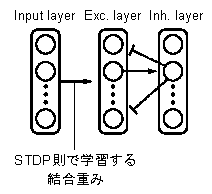
\includegraphics[scale=1.5]{figs/diehl.pdf}
    \caption{(Diehl \& Cook, 2015)で提案されたネットワーク.  1層目が入力層、2層目が興奮性ニューロン層と抑制性ニューロン層から構成されます。興奮性ニューロンと抑制性ニューロンの間の結合重みは固定で、入力層から興奮性ニューロン層へ投射される結合重みをSTDP則で学習します。}
    \label{fig:diehl}
\end{figure}

\subsection{ニューロンとシナプスのモデル}
ニューロンとシナプスのモデルとしてはConductance-basedモデルを用いています. 
\subsubsection{ニューロンのモデル}
興奮性ニューロンと抑制性ニューロンの膜電位$V$は次の式に従います. 
\begin{equation}
\tau \frac{d V}{d t}=\left(E_{\text {rest}}-V\right)+g_{e}\left(E_{\text {exc}}-V\right)+g_{i}\left(E_{\text {inh}}-V\right)    
\end{equation}
これは通常のConductance-basedモデルと同じ式ですが, ネットワークの発火率を一定に保つため, 興奮性ニューロンの膜電位の発火閾値は発火のたびに$\theta=0.05 $mV上昇するとします. 発火の無い場合は時定数$10^7$ msで減衰します. 著者実装では350 ms間, 画像をエンコードしたスパイク列を入力し, 変数をリセットするために150 ms間, 何も入力しないブランク期間を設定しています. この間に膜電位等は全てリセットされますが, 発火閾値のみ, 少し減衰するだけに留まります. さらに, 興奮性ニューロンの発火数が少ない場合には, 入力のポアソンスパイクの発火率を上げ, 再度同じ画像を提示します. \par
また, 興奮性ニューロンの膜電位の時定数としては生理学的に逸脱した100 msという値を用いています. これは時定数を大きくすることで, 多くのスパイク入力を積分することができ, ノイズによる影響を減らすことができると説明されています. \par
まず、準備としてこのようなニューロンを実装しておきます\footnote{コードは\texttt{./TrainingSNN/Models/Neurons.py}に含まれます. }. コード自体は2章で紹介したConductance-based LIFに修正を加えたものです。
\begin{minted}[frame=lines, framesep=2mm, baselinestretch=1.2, bgcolor=shadecolor,fontsize=\small]{python}
class DiehlAndCook2015LIF:
    def __init__(self, N, dt=1e-3, tref=5e-3, tc_m=1e-1,
                 vrest=-65, vreset=-65, init_vthr=-52, vpeak=20,
                 theta_plus=0.05, theta_max=35, tc_theta=1e4,
                 e_exc=0, e_inh=-100):
        self.N = N
        self.dt = dt
        self.tref = tref
        self.tc_m = tc_m 
        self.vreset = vreset
        self.vrest = vrest
        self.init_vthr = init_vthr
        self.theta = np.zeros(N)
        self.theta_plus = theta_plus
        self.theta_max = theta_max
        self.tc_theta = tc_theta
        self.vpeak = vpeak

        self.e_exc = e_exc \section{興奮性シナプスの平衡電位}
        self.e_inh = e_inh \section{抑制性シナプスの平衡電位}
        
        self.v = self.vreset*np.ones(N)
        self.vthr = self.init_vthr
        self.v_ = None
        self.tlast = 0
        self.tcount = 0
    
    def initialize_states(self, random_state=False):
        if random_state:
            self.v = self.vreset + \ 
                     np.random.rand(self.N)*(self.vthr-self.vreset) 
        else:
            self.v = self.vreset*np.ones(self.N)
        self.vthr = self.init_vthr
        self.theta = np.zeros(self.N)
        self.tlast = 0
        self.tcount = 0
        
    def __call__(self, g_exc, g_inh):
        I_synExc = g_exc*(self.e_exc - self.v) 
        I_synInh = g_inh*(self.e_inh - self.v)
        dv = (self.vrest - self.v + I_synExc + I_synInh) / self.tc_m
        v = self.v+((self.dt*self.tcount)>(self.tlast+self.tref))*dv*self.dt
        
        s = 1*(v>=self.vthr) #発火時は1, その他は0の出力
        
        \section{閾値の更新}
        theta = (1-self.dt/self.tc_theta)*self.theta + self.theta_plus*s
        self.theta = np.clip(theta, 0, self.theta_max)
        self.vthr = self.theta + self.init_vthr
        
        self.tlast = self.tlast*(1-s) + self.dt*self.tcount*s
        v = v*(1-s) + self.vpeak*s #閾値を超えると膜電位をvpeakにする
        self.v_ = v #発火時の電位も含めて記録するための変数
        self.v = v*(1-s) + self.vreset*s  #発火時に膜電位をリセット
        self.tcount += 1
        
        return s 
\end{minted}
追加した部分は閾値の更新のところです。最終的な閾値は\texttt{self.theta}と\texttt{self.init\_vthr}を加算した\texttt{self.vthr}を用います。変動するのは\texttt{self.theta}ですが、これはスパイクトレースと同様の実装をしています。ただし、閾値が上がりすぎることを防ぐため、上限を\texttt{self.theta\_max}として\texttt{np.clip()}により制限しています。

\subsubsection{シナプスのモデル}
シナプスにはConductance-basedの単一指数関数型シナプス(single exponential synapse)を用いています. スパイクが入るとコンダクタンス$g$は$w$だけあがり, その他では以下のように減衰します
\begin{equation}
\tau_{x} \frac{dg_x}{d t}=-g_x    
\end{equation}
ただし、$x=e, i$で、それぞれ興奮性、抑制性を意味する添え字です. なお、この実装自体は第2章で述べたものと変わりません. 

\subsection{興奮性ニューロンのラベリング}
このネットワークには出力層がなく, 通常とは異なる形式で画像を分類しています. まず, 訓練時において興奮性ニューロンの活動を全て記録します. 次に, 画像に元々されていたラベルを用いて, 興奮性の各ニューロンの各ラベルの画像への平均発火数を計算します. このとき, 各ニューロンにおいて最も発火数が多かったラベルを求め, そのラベルを各ニューロンに割り当てます. そして, 割り当てたラベルを用い, 入力画像に対する各ラベルに割り当てられたニューロンの平均発火数を求めます. このとき平均発火数が最も高いニューロン群のラベルが, 入力画像の予測ラベルとなります. また, 推論時には訓練時においてニューロンに割り当てたラベルを用います.\par
それではニューロンへラベルを割り当てる関数(\texttt{assign\_labels})を実装してみましょう\footnote{以降のコードは特に明記が無い限り\texttt{./TrainingSNN/LIF\_WTA\_STDP\_MNIST.py}に含まれます。また一部、BindsNETの実装を参考にしています。}。\texttt{assign\_labels}は5つの変数を引数に取ります。\texttt{spikes}は, サイズが\texttt{(n\_samples, n\_neurons)}の2次元配列で、各サンプルにおいて各興奮性ニューロンが何回発火したかを記録したものです。 \texttt{labels}はサイズが\texttt{(n\_samples, )}の配列で、各サンプルの教師ラベルを表します。\texttt{n\_labels}はラベルの数です。今回はMNISTなので10個です。 \texttt{rates}はサイズが\texttt{(n\_samples, n\_neurons)}の配列で、各興奮性ニューロンの各ラベルに対する発火率を表します。\texttt{rates}は2度目の計算以降に引数として渡すと、過去の\texttt{rates}と\texttt{alpha}によって調整される割合で指数平均を取ります。
\begin{minted}[frame=lines, framesep=2mm, baselinestretch=1.2, bgcolor=shadecolor,fontsize=\small]{python}
def assign_labels(spikes, labels, n_labels, rates=None, alpha=1.0):
    n_neurons = spikes.shape[1] 
    
    if rates is None:        
        rates = np.zeros((n_neurons, n_labels)).astype(np.float32)
    
    \section{時間の軸でスパイク数の和を取る}
    for i in range(n_labels):
        \section{サンプル内の同じラベルの数を求める}
        n_labeled = np.sum(labels == i).astype(np.int16)
    
        if n_labeled > 0:
            \section{label == iのサンプルのインデックスを取得}
            indices = np.where(labels == i)[0]
            
            \section{label == iに対する各ニューロンごとの平均発火率を計算}
            #(前回の発火率との移動平均)
            rates[:, i] = alpha*rates[:, i] + \ 
                          (np.sum(spikes[indices], axis=0)/n_labeled)
    
    sum_rate = np.sum(rates, axis=1)
    sum_rate[sum_rate==0] = 1
    \section{クラスごとの発火頻度の割合を計算する}
    proportions = rates / np.expand_dims(sum_rate, 1) \section{(n_neurons, n_labels)}
    proportions[proportions != proportions] = 0  \section{Set NaNs to 0}
    
    \section{最も発火率が高いラベルを各ニューロンに割り当てる (n_neurons,)}
    assignments = np.argmax(proportions, axis=1).astype(np.uint8) 

    return assignments, proportions, rates
\end{minted}
ここで\texttt{assignments}はサイズが\texttt{(n\_neurons,)}の配列で、各ニューロンに割り当てられたラベルを表します。これを用いて、各サンプルに対してラベルを予測する関数\texttt{prediction}を実装しましょう。
\begin{minted}[frame=lines, framesep=2mm, baselinestretch=1.2, bgcolor=shadecolor,fontsize=\small]{python}
def prediction(spikes, assignments, n_labels):    
    n_samples = spikes.shape[0]
    
    \section{各サンプルについて各ラベルの発火率を見る}
    rates = np.zeros((n_samples, n_labels)).astype(np.float32)
    
    for i in range(n_labels):
        \section{各ラベルが振り分けられたニューロンの数}
        n_assigns = np.sum(assignments == i).astype(np.uint8)
    
        if n_assigns > 0:
            \section{各ラベルのニューロンのインデックスを取得}
            indices = np.where(assignments == i)[0]
    
            \section{各ラベルのニューロンのレイヤー全体における平均発火数を求める}
            rates[:, i] = np.sum(spikes[:, indices], axis=1) / n_assigns
    
    \section{レイヤーの平均発火率が最も高いラベルを出力}
    return np.argmax(rates, axis=1).astype(np.uint8) \section{(n_samples, )}
\end{minted}
\texttt{prediction}は3つの引数, \texttt{spikes}, \texttt{assignments}, \texttt{n\_labels}を取ります。これらはそれぞれ先ほど説明した同名の配列と同じです。そして、各ラベルに紐づけられたニューロンごとに平均発火数を計算し、最も平均発火数の多かったラベルを入力サンプルのラベルとします。
\subsection{MNISTデータセットのスパイク列への変換}
入力として用いるために、MNISTデータセットをスパイク列へ変換する関数を書きましょう。MNISTデータセットを読み込む関数を別に書いても良いですが、煩雑となるため、ANNのライブラリに付属するデータ読み込み関数を利用してみます。ここでは例としてChainerの\texttt{chainer.datasets.get\_mnist()}を用いますが、他のライブラリでも大きな修正をすることなく実装できると思います。
\begin{minted}[frame=lines, framesep=2mm, baselinestretch=1.2, bgcolor=shadecolor,fontsize=\small]{python}
def online_load_and_encoding_dataset(dataset, i, dt, n_time, max_fr=32,
                                     norm=196):
    fr_tmp = max_fr*norm/np.sum(dataset[i][0])
    fr = fr_tmp*np.repeat(np.expand_dims(dataset[i][0],
                                         axis=0), n_time, axis=0)
    input_spikes = np.where(np.random.rand(n_time, 784) < fr*dt, 1, 0)
    input_spikes = input_spikes.astype(np.uint8)

    return input_spikes
\end{minted}
この関数の使用例と, スパイク列への変換が正しく行われているかを確認するコードは次のようになります。
\begin{minted}[frame=lines, framesep=2mm, baselinestretch=1.2, bgcolor=shadecolor,fontsize=\small]{python}
import chainer
dt = 1e-3; t_inj = 0.350; nt_inj = round(t_inj/dt)
train, _ = chainer.datasets.get_mnist() \section{ChainerによるMNISTデータの読み込み}
input_spikes = online_load_and_encoding_dataset(dataset=train, i=0,
                                                dt=dt, n_time=nt_inj)
\section{描画}
plt.imshow(np.reshape(np.sum(input_spikes, axis=0), (28, 28)),
           cmap="gray")
plt.show()
\end{minted}
ここでスパイク列を時間的に加算し、28$\times$28の配列に変換した後に描画をしています。結果は図\ref{fig:jitteredMNIST}のようになります。
\begin{figure}[htbp]
    \centering
    \includegraphics[scale=0.4]{figs/five.pdf}
    \caption{スパイク列に変換したMNISTデータの例(5).}
    \label{fig:jitteredMNIST}
\end{figure}

\subsection{ネットワークの実装}
それではネットワークを実装してみましょう。長いですが、それぞれの部分はこれまでの実装の組み合わせです。ただし、著者実装におけるハイパーパラメータでは正常に学習が進まなかったので、各ハイパーパラメータの値は変更しています\footnote{そもそも論文にハイパーパラメータが書いておらず、著者実装のコードを読むしかありません。}。
\begin{minted}[frame=lines, framesep=2mm, baselinestretch=1.2, bgcolor=shadecolor,fontsize=\small]{python}
class DiehlAndCook2015Network:
    def __init__(self, n_in=784, n_neurons=100, wexc=2.25, winh=0.875,
                 dt=1e-3, wmin=0.0, wmax=5e-2, lr=(1e-2, 1e-4),
                 update_nt=100):
        self.dt = dt
        self.lr_p, self.lr_m = lr
        self.wmax = wmax
        self.wmin = wmin
        self.n_neurons = n_neurons
        self.n_in = n_in
        self.norm = 0.1
        self.update_nt = update_nt

        \section{Neurons}
        self.exc_neurons = DiehlAndCook2015LIF(n_neurons, dt=dt, tref=5e-3,
                                               tc_m=1e-1,
                                               vrest=-65, vreset=-65, 
                                               init_vthr=-52,
                                               vpeak=20, theta_plus=0.05,
                                               theta_max=35,
                                               tc_theta=1e4,
                                               e_exc=0, e_inh=-100)

        self.inh_neurons = ConductanceBasedLIF(n_neurons, dt=dt, tref=2e-3,
                                               tc_m=1e-2,
                                               vrest=-60, vreset=-45,
                                               vthr=-40, vpeak=20,
                                               e_exc=0, e_inh=-85)
        \section{Synapses}
        self.input_synapse = SingleExponentialSynapse(n_in, dt=dt, td=1e-3)
        self.exc_synapse = SingleExponentialSynapse(n_neurons, dt=dt, td=1e-3)
        self.inh_synapse = SingleExponentialSynapse(n_neurons, dt=dt, td=2e-3)
        
        self.input_synaptictrace = SingleExponentialSynapse(n_in, dt=dt,
                                                            td=2e-2)
        self.exc_synaptictrace = SingleExponentialSynapse(n_neurons, dt=dt,
                                                          td=2e-2)
        
        \section{Connections (重みの初期化)}
        initW = 1e-3*np.random.rand(n_neurons, n_in)
        self.input_conn = FullConnection(n_in, n_neurons,
                                         initW=initW)
        self.exc2inh_W = wexc*np.eye(n_neurons)
        self.inh2exc_W = (winh/n_neurons)*(np.ones((n_neurons, n_neurons)) \
                          - np.eye(n_neurons))
        
        self.delay_input = DelayConnection(N=n_neurons, delay=5e-3, dt=dt)
        self.delay_exc2inh = DelayConnection(N=n_neurons, delay=2e-3, dt=dt)

        self.g_inh = np.zeros(n_neurons)
        
        self.tcount = 0

        self.s_in_ = np.zeros((self.update_nt, n_in)) 
        self.s_exc_ = np.zeros((n_neurons, self.update_nt))
        self.x_in_ = np.zeros((self.update_nt, n_in)) 
        self.x_exc_ = np.zeros((n_neurons, self.update_nt))
        
    \section{スパイクトレースのリセット}
    def reset_trace(self):
        self.s_in_ = np.zeros((self.update_nt, self.n_in)) 
        self.s_exc_ = np.zeros((self.n_neurons, self.update_nt))
        self.x_in_ = np.zeros((self.update_nt, self.n_in)) 
        self.x_exc_ = np.zeros((self.n_neurons, self.update_nt))
        self.tcount = 0
    
    \section{状態の初期化}
    def initialize_states(self):
        self.exc_neurons.initialize_states()
        self.inh_neurons.initialize_states()
        self.delay_input.initialize_states()
        self.delay_exc2inh.initialize_states()
        self.input_synapse.initialize_states()
        self.exc_synapse.initialize_states()
        self.inh_synapse.initialize_states()
        
    def __call__(self, s_in, stdp=True):
        \section{入力層}
        c_in = self.input_synapse(s_in)
        x_in = self.input_synaptictrace(s_in)
        g_in = self.input_conn(c_in)

        \section{興奮性ニューロン層}
        s_exc = self.exc_neurons(self.delay_input(g_in), self.g_inh)
        c_exc = self.exc_synapse(s_exc)
        g_exc = np.dot(self.exc2inh_W, c_exc)
        x_exc = self.exc_synaptictrace(s_exc)

        \section{抑制性ニューロン層        }
        s_inh = self.inh_neurons(self.delay_exc2inh(g_exc), 0)
        c_inh = self.inh_synapse(s_inh)
        self.g_inh = np.dot(self.inh2exc_W, c_inh)

        if stdp:
            \section{スパイク列とスパイクトレースを記録}
            self.s_in_[self.tcount] = s_in
            self.s_exc_[:, self.tcount] = s_exc
            self.x_in_[self.tcount] = x_in 
            self.x_exc_[:, self.tcount] = x_exc
            self.tcount += 1

            \section{Online STDP}
            if self.tcount == self.update_nt:
                W = np.copy(self.input_conn.W)
                
                \section{postに投射される重みが均一になるようにする}
                W_abs_sum = np.expand_dims(np.sum(np.abs(W), axis=1), 1)
                W_abs_sum[W_abs_sum == 0] = 1.0
                W *= self.norm / W_abs_sum
                
                \section{STDP則}
                dW = self.lr_p*(self.wmax-W)*np.dot(self.s_exc_, self.x_in_)
                dW -= self.lr_m*W*np.dot(self.x_exc_, self.s_in_)
                clipped_dW = np.clip(dW / self.update_nt, -5e-2, 5e-2)
                self.input_conn.W = np.clip(W + clipped_dW,
                                            self.wmin, self.wmax)
                self.reset_trace() \section{スパイク列とスパイクトレースをリセット}
        
        return s_exc
\end{minted}
ここで\texttt{\_\_call\_\_()}関数は入力スパイク列\texttt{s\_in}とSTDP則による学習をするかどうかのBoolean変数である\texttt{stdp}の2つの値を引数とします。\texttt{stdp}が\textttt{True}のとき、入力層と興奮性ニューロン層のスパイク列、スパイクトレースが記録され、\texttt{self.tcount}が\textttt{self.update\_nt}となったときにSTDP則による重みの更新が行われます。重みの更新の前に、興奮性ニューロンへ投射される重みの合計が\texttt{self.norm}となるように正規化をしています。また、ここでのSTDP則は重み依存的なものとしています。なお、重みの更新時に重みが
\texttt{self.wmin}と\texttt{self.wmax}範囲となるように\texttt{np.clip()}で制限をしています。
\subsection{学習イテレーションと結果の表示}
実際にシミュレーションをする部分を書いていきます。タイムステップは1 msとし、350 msの間は画像を変換したスパイク列を入力、150 msの間何も入力しない、というようにします。また、興奮性ニューロンの数は100個とし、訓練データのサンプル数は10000, エポック数は20とします。\par
なお、学習後にネットワークの評価をするために、このファイル内の関数を呼び出します。そのため、この部分は外部から呼び出されないように\texttt{if \_\_name\_\_ == '\_\_main\_\_':}と記述した中に書いておきます。
\begin{minted}[frame=lines, framesep=2mm, baselinestretch=1.2, bgcolor=shadecolor,fontsize=\small]{python}
if __name__ == '__main__':
    \section{350ms画像入力、150ms入力なしでリセットさせる(膜電位の閾値以外)}
    dt = 1e-3 \section{タイムステップ(sec)}
    t_inj = 0.350 \section{刺激入力時間(sec)}
    t_blank = 0.150 \section{ブランク時間(sec)}
    nt_inj = round(t_inj/dt)
    nt_blank = round(t_blank/dt)
    
    n_neurons = 100 \section{興奮性/抑制性ニューロンの数}
    n_labels = 10 \section{ラベル数}
    n_epoch = 20 \section{エポック数}
    
    n_train = 10000 \section{訓練データの数}
    update_nt = nt_inj \section{STDP則による重みの更新間隔}
    
    \section{ChainerによるMNISTデータの読み込み}
    train, _ = chainer.datasets.get_mnist()
    labels = np.array([train[i][1] for i in range(n_train)]) \section{ラベルの配列}
    
    \section{ネットワークの定義}
    network = DiehlAndCook2015Network(n_in=784, n_neurons=n_neurons,
                                      wexc=2.25, winh=0.875,
                                      dt=dt, wmin=0.0, wmax=0.1,
                                      lr=(1e-2, 1e-4),
                                      update_nt=update_nt)
    
    network.initialize_states() \section{ネットワークの初期化}

    spikes = np.zeros((n_train, n_neurons)).astype(np.uint8) \section{スパイク記録変数}
    accuracy_all = np.zeros(n_epoch) \section{訓練精度を記録する変数}
    blank_input = np.zeros(784) \section{ブランク入力}
    init_max_fr = 32 \section{初期のポアソンスパイクの最大発火率}
    
    \section{結果を保存するディレクトリ}
    results_save_dir = "./LIF_WTA_STDP_MNIST_results/"
    os.makedirs(results_save_dir, exist_ok=True) \section{ディレクトリが無ければ作成}
    
    \section{Simulation}
    for epoch in range(n_epoch):
        for i in tqdm(range(n_train)):
            max_fr = init_max_fr
            while(True):
                \section{入力スパイクをオンラインで生成}
                input_spikes = online_load_and_encoding_dataset(train, i, dt,
                                                                nt_inj,
                                                                max_fr)
                spike_list = [] \section{サンプルごとにスパイクを記録するリスト}
                \section{画像刺激の入力}
                for t in range(nt_inj):
                    s_exc = network(input_spikes[t], stdp=True)
                    spike_list.append(s_exc)
                
                \section{スパイク数を記録}
                spikes[i] = np.sum(np.array(spike_list), axis=0)
                
                \section{ブランク刺激の入力}
                for _ in range(nt_blank):
                    _ = network(blank_input, stdp=False)
    
                \section{スパイク数を計算}
                num_spikes_exc = np.sum(np.array(spike_list))
                \section{スパイク数が5より大きければ次のサンプルへ}
                if num_spikes_exc >= 5:
                    break
                else: \section{スパイク数が5より小さければ入力発火率を上げて再度刺激}
                    max_fr += 16
        
        \section{ニューロンを各ラベルに割り当てる}
        if epoch == 0:
            assignments, proportions, rates = assign_labels(spikes, labels,
                                                            n_labels)
        else:
            assignments, proportions, rates = assign_labels(spikes, labels,
                                                            n_labels, rates)
        print("Assignments:\n", assignments)
        
        \section{スパイク数の確認(正常に発火しているか確認)}
        sum_nspikes = np.sum(spikes, axis=1)
        mean_nspikes = np.mean(sum_nspikes).astype(np.float16)
        print("Ave. spikes:", mean_nspikes)
        print("Min. spikes:", sum_nspikes.min())
        print("Max. spikes:", sum_nspikes.max())
    
        \section{入力サンプルのラベルを予測する}
        predicted_labels = prediction(spikes, assignments, n_labels)
        
        \section{訓練精度を計算}
        accuracy = np.mean(np.where(labels==predicted_labels, 1, 0))
        print("epoch :", epoch, " accuracy :", accuracy)
        accuracy_all[epoch] = accuracy
        
        \section{学習率の減衰}
        network.lr_p *= 0.85
        network.lr_m *= 0.85
        
        \section{重みの保存(エポック毎)}
        np.save(results_save_dir+"weight_epoch"+str(epoch)+".npy",
                network.input_conn.W)
        
    \section{結果}
    plt.figure(figsize=(5,4))
    plt.plot(np.arange(1, n_epoch+1), accuracy_all*100,
             color="k")
    plt.xlabel("Epoch")
    plt.ylabel("Train accuracy (%)")
    plt.savefig(results_save_dir+"accuracy.png")
    
    np.save(results_save_dir+"assignments.npy", assignments)
    np.save(results_save_dir+"weight.npy", network.input_conn.W)
    np.save(results_save_dir+"exc_neurons_theta.npy",
            network.exc_neurons.theta)
\end{minted}
シミュレーション部は入れ子状のループとなっています。\texttt{while}によるループは, サンプルを入力した時に興奮性ニューロン全体の発火数が5を超えない限り, 入力の発火率を増加させて再度スパイク列を入力する、ということを行います。\par
各エポック終了時には刺激時の興奮性ニューロンの発火情報から、興奮性ニューロンの各ラベルへの割り当てと各サンプルのラベルの予測、および訓練精度の計算を行います。最後にSTDP則における学習率を減衰させます。\par
学習が終了した後は訓練精度の変化と各ニューロンに割り当てたラベル(\texttt{assignments})、入力層から興奮性ニューロンへの結合重み、興奮性ニューロンの閾値を保存しておきます。なお、学習時における訓練精度の変化は図\ref{fig:MNISTaccuracy}のようになりました。
\begin{figure}[htbp]
    \centering
    \includegraphics[scale=0.5]{figs/accuracy.pdf}
    \caption{訓練時の精度の変化. 最終的な訓練精度は69.9\%となりました。}
    \label{fig:MNISTaccuracy}
\end{figure}

\subsection{ネットワークの評価}
学習後のネットワークを学習に用いなかったテストデータで評価してみましょう。
\footnote{コードは\texttt{./TrainingSNN/LIF\_WTA\_STDP\_MNIST\_evaluation.py}です。}。ほぼネットワークの学習の際に記述したコードを流用するだけです。まず、学習後の重みを読み込んで、テストデータ(1000サンプル)を入力し、それに対するスパイクを記録します。次に訓練時に行った各ニューロンのラベルへの割り当てを用いて各サンプルのラベルを予測し、実際のラベルと比較し、推論精度を計算します。
\begin{minted}[frame=lines, framesep=2mm, baselinestretch=1.2, bgcolor=shadecolor,fontsize=\small]{python}
import chainer
from LIF_WTA_STDP_MNIST import online_load_and_encoding_dataset, prediction
from LIF_WTA_STDP_MNIST import DiehlAndCook2015Network

\section{350ms画像入力、150ms入力なしでリセットさせる(膜電位の閾値以外)}
dt = 1e-3 \section{タイムステップ(sec)}
t_inj = 0.350 \section{刺激入力時間(sec)}
t_blank = 0.150 \section{ブランク時間(sec)}
nt_inj = round(t_inj/dt)
nt_blank = round(t_blank/dt)

n_neurons = 100 #興奮性/抑制性ニューロンの数
n_labels = 10 #ラベル数

n_train = 1000 \section{訓練データの数}
update_nt = nt_inj \section{STDP則による重みの更新間隔}

_, test = chainer.datasets.get_mnist() \section{ChainerによるMNISTデータの読み込み}
labels = np.array([test[i][1] for i in range(n_train)]) \section{ラベルの配列}

\section{結果が保存されているディレクトリ}
results_save_dir = "./LIF_WTA_STDP_MNIST_results/"

\section{ネットワークの定義}
network = DiehlAndCook2015Network(n_in=784, n_neurons=n_neurons,
                                  wexc=2.25, winh=0.875,
                                  dt=dt, wmin=0.0, wmax=0.1,
                                  lr=(1e-2, 1e-4),
                                  update_nt=update_nt)

network.initialize_states() \section{ネットワークの初期化}

\section{重みと閾値のload}
network.input_conn.W = np.load(results_save_dir+"weight.npy")
network.exc_neurons.theta = np.load(results_save_dir+"exc_neurons_theta.npy")
network.exc_neurons.theta_plus = 0 \section{閾値が上昇しないようにする}

#スパイクを記録する変数
spikes = np.zeros((n_train, n_neurons)).astype(np.uint8)
blank_input = np.zeros(784) \section{ブランク入力}
init_max_fr = 32 \section{初期のポアソンスパイクの最大発火率}

for i in tqdm(range(n_train)):
    max_fr = init_max_fr
    while(True):
        \section{入力スパイクをオンラインで生成}
        input_spikes = online_load_and_encoding_dataset(test, i, dt,
                                                        nt_inj, max_fr)
        spike_list = [] \section{サンプルごとにスパイクを記録するリスト}
        \section{画像刺激の入力}
        for t in range(nt_inj):
            s_exc = network(input_spikes[t], stdp=False)
            spike_list.append(s_exc)
        
        spikes[i] = np.sum(np.array(spike_list), axis=0) \section{スパイク数を記録}
        
        \section{ブランク刺激の入力}
        for _ in range(nt_blank):
            _ = network(blank_input, stdp=False)

        num_spikes_exc = np.sum(np.array(spike_list)) \section{スパイク数を計算}
        if num_spikes_exc >= 5: \section{スパイク数が5より大きければ次のサンプルへ}
            break
        else: \section{スパイク数が5より小さければ入力発火率を上げて再度刺激}
            max_fr += 16
            
\section{入力サンプルのラベルを予測する}
assignments = np.load(results_save_dir+"assignments.npy")
predicted_labels = prediction(spikes, assignments, n_labels)

\section{訓練精度を計算}
accuracy = np.mean(np.where(labels==predicted_labels, 1, 0))
print("Test accuracy :", accuracy)
\end{minted}
実行した結果、\colorbox{shadecolor}{\texttt{Test accuracy : 0.653}}となり、テストデータ(1000サンプル)での精度は65.3\%となりました。100個のニューロンを学習させた際の論文における精度が約85\%であるので、それに比べるとかなり低い値です。これには学習データを少なくしている、ハイパーパラメータを著者実装とは異なるものにしているということなどが原因であると考えられます。

\subsection{興奮性ニューロンの受容野の描画}
最後に、学習後の入力層から興奮性ニューロン層へのシナプス重みを描画してみましょう\footnote{コードは\texttt{./TrainingSNN/LIF\_WTA\_STDP\_MNIST\_visualize\_weights.py}です。}。各興奮性ニューロンへ投射する784個のシナプス重みを28$\times$28に\texttt{reshape}して描画するだけです。
\begin{minted}[frame=lines, framesep=2mm, baselinestretch=1.2, bgcolor=shadecolor,fontsize=\small]{python}
epoch = 19
n_neurons = 100

\section{結果が保存されているディレクトリ}
results_save_dir = "./LIF_WTA_STDP_MNIST_results/"

input_conn_W = np.load(results_save_dir+"weight_epoch"+str(epoch)+".npy")
reshaped_W = np.reshape(input_conn_W, (n_neurons, 28, 28))

\section{描画}
fig = plt.figure(figsize=(6,6))
fig.subplots_adjust(left=0, right=1, bottom=0, top=1,
                    hspace=0.05, wspace=0.05)
row = col = np.sqrt(n_neurons)
for i in tqdm(range(n_neurons)):
  ax = fig.add_subplot(row, col, i+1, xticks=[], yticks=[])
  ax.imshow(reshaped_W[i], cmap="gray")
plt.savefig("weights_"+str(epoch)+".png")
plt.show()
\end{minted}
結果は図\ref{fig:Diehl_weights}のようになります。
\begin{figure}[htbp]
 \begin{minipage}{0.5\hsize}
  \begin{center}
   \includegraphics[width=60mm]{figs/weights_0.pdf}
  \end{center}
 \end{minipage}
 \begin{minipage}{0.5\hsize}
  \begin{center}
   \includegraphics[width=60mm]{figs/weights_19.pdf}
  \end{center}
 \end{minipage}
\caption{学習後の100個の興奮性ニューロンの重みを描画したもの。各数字に対応するフィルターが生まれていることが分かります。(左) 1エポック終了時の重み。受容野が生じつつあるのが分かります。(右) 20エポック終了時。一番上の段の10個のニューロンをラベルに割り当てた結果は``5, 2, 6, 3, 3, 9, 4, 3, 0, 2"となっており、受容野の見た目と一致しています。}
\label{fig:Diehl_weights}
\end{figure}
\end{document}
